\documentclass[]{beamer}
\mode<presentation>
{
% use attribute "dark" for dark theme
% use attribute "contrast" for maximum text contrast
\usetheme[]{wlansi}
\usefonttheme[onlymath]{serif}
\setbeamercovered{transparent}
}  

\usepackage{hyperref}
\usepackage[utf8]{inputenc}
\usepackage{mathptmx}
\usepackage{xmpmulti}
\usepackage[T1]{fontenc}
\usepackage[utf8]{inputenc}
\usepackage{cmap}
\usepackage{ifthen}
\usepackage{type1ec}
\usepackage{concrete}
\usepackage{tikz}
\usetikzlibrary{positioning,arrows,decorations.pathreplacing,decorations.text,shapes,calc,fit}
\DeclareFontFamily{T1}{ccr}{}
\DeclareFontShape{T1}{ccr}{m}{n}{<5><6><7><8><9><10>gen*eorm<10->eorm10}{}
\DeclareFontShape{T1}{ccr}{m}{sl}{<5><6><7><8><9><10>gen*eosl<10->eosl10}{}
\DeclareFontShape{T1}{ccr}{m}{it}{<->eoti10}{}
\DeclareFontShape{T1}{ccr}{m}{sc}{<->eocc10}{}
\DeclareFontShape{T1}{ccr}{bx}{n}{<->ssub*cmr/bx/n}{}
\DeclareFontShape{T1}{ccr}{bx}{sl}{<->ssub*cmr/bx/sl}{}
\DeclareFontShape{T1}{ccr}{bx}{it}{<->ssub*cmr/bx/it}{}
\DeclareFontShape{T1}{ccr}{sbc}{n}{<->ssubf*ecssdc10}{}
\usepackage[T1]{fontenc}
\renewcommand{\sfdefault}{\rmdefault}
\renewcommand{\familydefault}{\rmdefault}
\renewcommand{\bfdefault}{m}
\newcommand{\nodewatcher}{\emph{nodewatcher }}
\newcommand{\wlanslovenija}{\emph{wlan slovenija }}

\newcommand{\ifstrempty}[3]{%
\def\reallyempty{}%
\def\ifarg{#1}%
\ifx\ifarg\reallyempty%
{#2}
\else
{#3}
\fi%
}

\newcommand{\wrapframe}[1]{
\begin{frame}
 #1
\end{frame}
}

\newenvironment{changemargin}[2]{%
\begin{list}{}{%
\setlength{\topsep}{0pt}%
\setlength{\leftmargin}{#1}%
\setlength{\rightmargin}{#2}%
\setlength{\listparindent}{\parindent}%
\setlength{\itemindent}{\parindent}%
\setlength{\parsep}{\parskip}%
}%
\item[]}{\end{list}}

\newcommand{\simpleslide}[3]{\wrapframe{
\ifstrempty{#1}{\vbox{ \ } 

}{
{\footnotesize #1}
} \vfill

\begin{center}
#2
\end{center}
\vfill
\ifstrempty{#3}{ \ }{
\begin{flushright}
{\footnotesize #3}
\end{flushright}
}
}}

\newcommand{\simpleslideimage}[2]{\wrapframe{
\begin{center}
\includegraphics[width=0.8\paperwidth,height=0.6\paperheight,keepaspectratio]{#1}
\\ {\footnotesize #2}
\end{center}}
}

\newcommand{\fullslideimage}[1]{
\begin{frame}[plain]
\begin{changemargin}{-1cm}{-1cm}
\begin{center}
\includegraphics[width=\paperwidth,height=\paperheight,keepaspectratio]{#1}
\end{center}
\end{changemargin}
\end{frame}
}

\newcommand{\rightfooter}[1]{\vfill\hfill #1}

\newlength{\pheight}
\newlength{\pwidth}
\setlength{\pheight}{0.8\paperheight}
\setlength{\pwidth}{0.8\paperwidth}

\title{Osnove WiFi in računalniška omrežja}

%\subtitle{}

%\author{}

%\institute{}

\date[]{1.0
}

\tikzstyle{vertex}=[circle,text=blue!75,fill=blue!25,minimum size=20pt,inner sep=0pt]
\tikzstyle{selected vertex} = [vertex, fill=red!24, text=red]
\tikzstyle{edge} = [draw=black,thick,-]
\tikzstyle{weight} = [font=\scriptsize]
\tikzstyle{selected edge} = [draw,line width=5pt,-,red!50]
\tikzstyle{destination} = [vertex,fill=orange!24, text=orange]

\pgfdeclarelayer{background}
\pgfsetlayers{background,main}

\begin{document}

% makes a title slide
\maketitle

\simpleslideimage{images/wr741nd-4v20-4.jpg}{Router TP-Link WR741ND}

\simpleslide{WR741ND}{
\begin{itemize}
\item CPU -- Atheros AR9331 @ 350 MHz
\item RAM -- 32 MB
\item flash -- 4 MB
\item LAN -- 4x 100 Mbps Auto MDI/MDIX
\item WAN -- 1x 100 Mbps Auto MDI/MDIX
\item WiFi -- 802.11 b/g/n 150 Mbps (130 Mbps realno) \\ 20 dBm -- 100 mW @ 2.4 GHz
\end{itemize}
}{}

\simpleslideimage{images/TP-LINK-serial.pdf}{Vezje za priklop na serijski port (voltage level shifter).}

\simpleslide{Izbira lokacije in antene za \wlanslovenija točko.}{
\begin{itemize}
\item Lokacija z čim večjim vidnim poljem (streha, okenska polica, fasada \dots).
\item Območje potencialnih uporabnikov (naselja, parki, javne površine, hribi \dots).
\item Primerna antena glede na ovire (omni za streho, panel za fasado, yagi za usmerjene povezave \dots).
\item Povezovanje z drugimi točkami.
\end{itemize}
}{}

\simpleslide{WiFi zakonodaja.}{Omejena izotropsko ekvivalenta izsevana moč -- EIRP.}{Router (dBm) + antena (dBi).}

\simpleslide{WiFi zakonodaja.}{
20 dBm EIRP @ 2.4 GHz. \\
23 dBm EIRP @ 5150--5350 MHz (v stavbah). \\
30 dBm EIRP @ 5475--5725 MHz.}{}

\simpleslide{}{Veliko malih šepetalcev.}{Namesto velikih oddajnih stolpov.}

\simpleslide{Namesto velikih oddajnih moči.}{}{Namesto zelo stabilnih in zelo kompleksnih in zato dragih vozlišč.}

\simpleslide{Veliko malih šepetalcev.}{Poceni in zamenljivi.}{Interoperabilni.}

\simpleslide{}{Ena točka. \\ $\downarrow$ \\ Dve točki -- povezava. \\ $\downarrow$ \\ Več točk -- omrežje.}{}

\simpleslide{Omrežje.}{Internet.}{Splet.}

\simpleslide{}{Omrežne plasti.}{Lego kocke.}

\simpleslideimage{images/legostack.jpg}{}

\simpleslide{Modularnost.}{Razširljivost.}{Interopabilnost.}

\simpleslide{Plasti (na Internetu).}{
\begin{enumerate}
\item Povezavna plast.
\item Internetna plast.
\item Transportna plast.
\item Aplikacijska plast.
\end{enumerate}}{}

\simpleslide{Povezavna plast.}{WiFi. Ethernet. xDSL. Tuneli.}{Lokalno (vidno) območje.}

\simpleslide{Internetna plast.}{Internet Protocol (IPv4, IPv6).}{Povezuje lokalna omrežja med seboj.}

\fullslideimage{images/internetmap.png}

\simpleslide{Transportna plast.}{TCP, UDP.}{Skrbi za end-to-end komunikacijo med napravami na Internetu.}

\simpleslide{Aplikacijska plast.}{HTTP, FTP, SMTP, IMAP, POP3, Skype, Bittorrent \dots}{HTTP = splet. SMTP, IMAP, POP3 = elektronska pošta.}

\simpleslide{\wlanslovenija omrežje.}{''Lokalno`` omrežje na nivoju države. :-)}{}

\simpleslideimage{images/network_topology.png}{Izsek grafa topologije \wlanslovenija omrežja.}

\simpleslide{Topologija omrežja.}{Dostopovne točke vs. mesh omrežje.}{}

\simpleslide{Omrežje dostopovne točke.}{

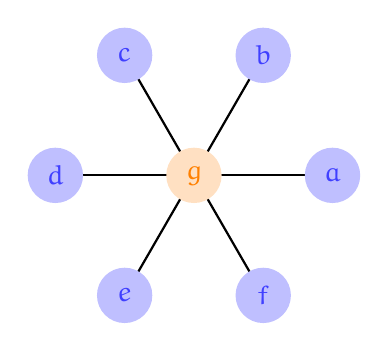
\begin{tikzpicture}[scale=1.1,auto,swap] 
  \foreach \name [count=\xi] in {a, b, c, d, e, f}
    \path[edge] (0,0) -- (-60+\xi*60:1.6) node[vertex] {$\name$};

  \node[destination] (g) at (0,0) {$g$};
\end{tikzpicture}

}{Zvezdasto.}

\simpleslide{Mesh omrežje.}{

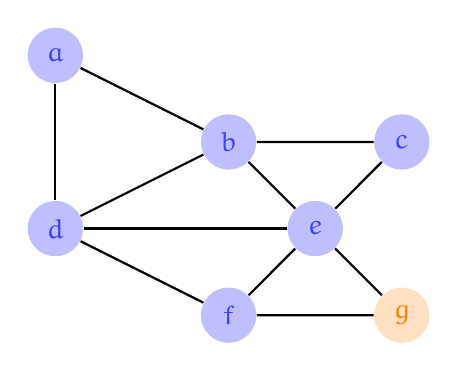
\begin{tikzpicture}[scale=1.1,auto,swap]
  \foreach \pos / \name in {{(0,2)/a}, {(2,1)/b}, {(4,1)/c},
                            {(0,0)/d}, {(3,0)/e}, {(2,-1)/f}}
    \node[vertex] (\name) at \pos {$\name$};
  
  \node[destination] (g) at (4,-1) {$g$};
  
  % Connect vertices with edges
  \foreach \source / \dest in {b/a, c/b, d/a, d/b,
                               e/b, e/c, e/d,
                               f/d, f/e, g/e, g/f}
      \path[edge] (\source) -- (\dest);
\end{tikzpicture}

}{Peer-to-peer.}

\simpleslide{Usmerjanje v omrežjih.}{Dinamični usmerjevalni protokoli.}{Statično usmerjanje.}

\simpleslide{}{Dinamično usmerjanje v WiFi mesh omrežjih.}{V \wlanslovenija omrežju uporabljamo protokol OLSR.}

\simpleslide{Najkvalitetnejša (najkrajša) pot od točke $a$ do $g$.}{

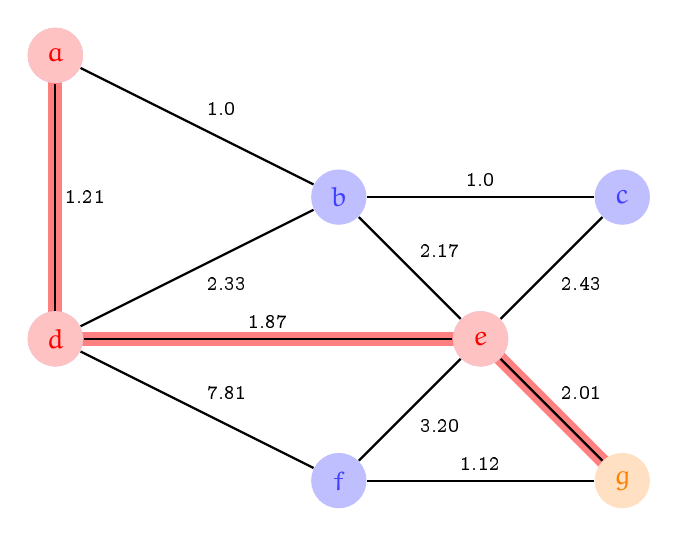
\begin{tikzpicture}[scale=1.8,auto,swap]
  \foreach \pos / \name in {{(0,2)/a}, {(2,1)/b}, {(4,1)/c},
                            {(0,0)/d}, {(3,0)/e}, {(2,-1)/f}}
    \node[vertex] (\name) at \pos {$\name$};
  
  \node[destination] (g) at (4,-1) {$g$};
  
  % Connect vertices with edges and draw weights
  \foreach \source / \dest / \weight in {b/a/$1.0$, c/b/$1.0$, d/a/$1.21$, d/b/$2.33$,
                                         e/b/$2.17$, e/c/$2.43$, e/d/$1.87$,
                                         f/d/$7.81$, f/e/$3.20$,
                                         g/e/$2.01$, g/f/$1.12$}
      \path[edge] (\source) -- node[weight] {$\weight$} (\dest);
  
  \foreach \vertex in {a,d,e}
    \path<2-> node[selected vertex] at (\vertex) {$\vertex$};
  
  \begin{pgfonlayer}{background}
    \foreach \source / \dest in {a/d,d/e,e/g}
      \path<2->[selected edge] (\source.center) -- (\dest.center);
  \end{pgfonlayer}
\end{tikzpicture}

}{}

\end{document}
